\documentclass[12pt, conference]{IEEEtran}
%\IEEEoverridecommandlockouts
% The preceding line is only needed to identify funding in the first footnote. If that is unneeded, please comment it out.
\usepackage{cite}
\usepackage{amsmath,amssymb,amsfonts}
\usepackage{algorithmic}
\usepackage{graphicx}
\usepackage{textcomp}
\usepackage{tikz}

\graphicspath{/}

\def\BibTeX{{\rm B\kern-.05em{\sc i\kern-.025em b}\kern-.08em
    T\kern-.1667em\lower.7ex\hbox{E}\kern-.125emX}}
\begin{document} 

\title{Alignment of Probabilistic Sequences Using Hidden Markov Models}

\author{\IEEEauthorblockN{Theodore Morley}
\IEEEauthorblockA{260621657 -- McGill University -- December 11th, 2017}}

\maketitle

\begin{abstract}
\textbf{Alignment of query sequences to probabilistic genome sequences has important applications in comparing modern data against computationally inferred ancestral sequences. Approaches using Hidden Markov Models to simulate the entire genome are too computationally expensive for this task, so heuristic approximations to reduce the search space are explored in this paper, and they have limited success in finding the location of modified sequences from the Boreoeutherian ancestor's genome.}
\end{abstract}

\begin{IEEEkeywords}
Hidden Markov Models, Probabilistic Sequences, Ancestral Sequences, Simulated Annealing
\end{IEEEkeywords}

\section{\textbf{Introduction}}

Within the field of ancestral reconstruction, the techniques for inferring the genetic sequence of an ancestor of interest are frequently best estimates, and therefore the constructed genomes can often be defined by a probability distribution for each position in the genome, giving the probability of any given nucleotide occupying the position.

Such a probabilistic genome sequence can be seen in the example in table 1.

Given this sequence, we would be interested in performing similar analyses that BLAST allows, in which we search a much shorter query sequence to find an alignment on a section of the genome. However, BLAST is not defined for probabilistic sequences such as this, and thus other approaches must be taken.


	\subsection{\textbf{The Tested Data}}
	
\begin{table}[htbp]
\centering
\caption{Example Probablistic Sequence}
\label{exprob}
\begin{tabular}{lllll}
  & 1    & 2 & 3   & ... \\
A & 0.75 & 0 & 0.5 &     \\
C & 0.25 & 0 & 0   &     \\
G & 0    & 0 & 0   &     \\
T & 0    & 1 & 0.5 &    
\end{tabular}
\end{table}

	The data used for testing and evaluation during the development of this algorithm is a computationally inferred segment of the Boreoeutherian ancestor's genome, with confidence values for each position. The probability of being any nucleotide other than the chosen one was evenly distributed amongst the remaining nucleotides.

	\subsection{\textbf{Optimal Alignment in a Probabilistic Setting?}}
	
	The first hurdle in finding an alignment against a probabilistic sequence is in fact defining what an optimal alignment even is in this context. In the non-probabilistic context, an optimal alignment could be defined as being the highest scoring alignment according to a scoring matrix. As a simple example, if matches within the alignment were defined as scoring +5, and mismatches as -4, the optimal alignment would be the one in which the query sequence lines up with the genome in such a way that the number of matches is maximized, and the number of mismatches is minimized.
	
	In a probabilistic setting, the notion of a match is not as well defined. If one position has an equal probability of being any nucleotide, how does one score an alignment of 'A' against that position?
	
	The approach in this paper is based off two main intuitions about this question:
	
	\begin{itemize}
		\item Given set scores for an alignment between two characters, the alignment with the higher probability should have the most impact on the resulting score.
		\item If a query sequence has evolved from a section of the genome sequence, then when we view the genome sequence as a Hidden Markov Model, in which each position is a state, and the emission probability is defined by the probability distribution at that position, then the query sequence should have a high likelihood of being generated by the genome model.
	\end{itemize}

	\subsection{\textbf{Hidden Markov Model Based Approaches}}
	
	Based off of these intuitions, I decided to explore the viability of using Hidden Markov Models to create optimal alignments of the query sequence.
	
	A Hidden Markov Model is a state based approach which aims to model sequences of unobserved states through information gathered from observations, whose probability depends on the underlying state structure. One of the appealing facets of the HMM approach is the existence of the Viterbi Algorithm[2], which allows us to find the most likely sequence of states to have produced a sequence of emissions. The hope I had for this approach was that I could use the Viterbi algorithm to find the most likely sequence of positions to have produced a given query sequence, and that this could be used to produce an exact alignment.
	
	In a first approach, I decided to adapt the idea of Profile Hidden Markov Models[3], which are a variant on HMM's used frequently in protein sequence homology detection, for example. The general idea I had was to create an HMM based off of the genome provided, with states for insertions, deletions, and matches, in which the match states would have their emission distribution determined by the probability distribution at the corresponding point in the genome.
	
	An example diagram of my original constructed HMM can below, where M* stands for a match state, I* an insertion, and D* a deletion:

\begin{center}
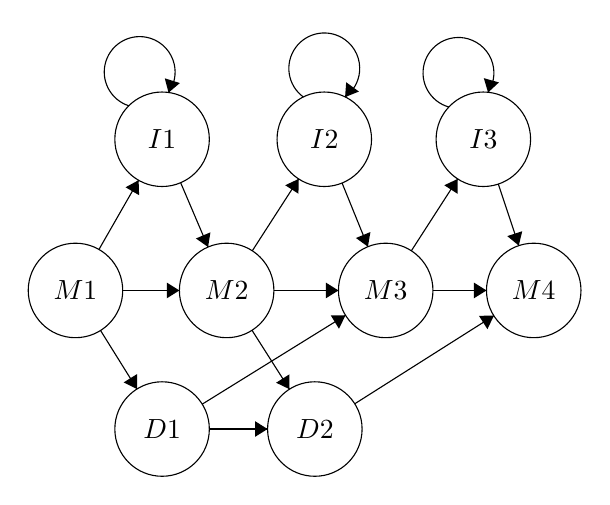
\begin{tikzpicture}[scale=0.2]
\tikzstyle{every node}+=[inner sep=0pt]
\draw [black] (10.7,-27.3) circle (3);
\draw (10.7,-27.3) node {$M1$};
\draw [black] (20.3,-27.3) circle (3);
\draw (20.3,-27.3) node {$M2$};
\draw [black] (30.4,-27.3) circle (3);
\draw (30.4,-27.3) node {$M3$};
\draw [black] (39.8,-27.3) circle (3);
\draw (39.8,-27.3) node {$M4$};
\draw [black] (16.2,-17.7) circle (3);
\draw (16.2,-17.7) node {$I1$};
\draw [black] (16.2,-36.1) circle (3);
\draw (16.2,-36.1) node {$D1$};
\draw [black] (25.9,-36.1) circle (3);
\draw (25.9,-36.1) node {$D2$};
\draw [black] (26.5,-17.7) circle (3);
\draw (26.5,-17.7) node {$I2$};
\draw [black] (36.6,-17.7) circle (3);
\draw (36.6,-17.7) node {$I3$};
\draw [black] (12.29,-29.84) -- (14.61,-33.56);
\fill [black] (14.61,-33.56) -- (14.61,-32.61) -- (13.76,-33.14);
\draw [black] (12.19,-24.7) -- (14.71,-20.3);
\fill [black] (14.71,-20.3) -- (13.88,-20.75) -- (14.74,-21.25);
\draw [black] (14.098,-15.576) arc (252.43495:-35.56505:2.25);
\fill [black] (16.61,-14.74) -- (17.33,-14.13) -- (16.37,-13.83);
\draw [black] (25.177,-15.02) arc (234:-54:2.25);
\fill [black] (27.82,-15.02) -- (28.7,-14.67) -- (27.89,-14.08);
\draw [black] (34.421,-15.655) arc (254.55605:-33.44395:2.25);
\fill [black] (36.9,-14.73) -- (37.59,-14.09) -- (36.63,-13.82);
\draw [black] (19.2,-36.1) -- (22.9,-36.1);
\fill [black] (22.9,-36.1) -- (22.1,-35.6) -- (22.1,-36.6);
\draw [black] (18.75,-34.52) -- (27.85,-28.88);
\fill [black] (27.85,-28.88) -- (26.91,-28.88) -- (27.43,-29.73);
\draw [black] (28.43,-34.5) -- (37.27,-28.9);
\fill [black] (37.27,-28.9) -- (36.32,-28.91) -- (36.86,-29.76);
\draw [black] (21.91,-29.83) -- (24.29,-33.57);
\fill [black] (24.29,-33.57) -- (24.28,-32.63) -- (23.44,-33.16);
\draw [black] (13.7,-27.3) -- (17.3,-27.3);
\fill [black] (17.3,-27.3) -- (16.5,-26.8) -- (16.5,-27.8);
\draw [black] (23.3,-27.3) -- (27.4,-27.3);
\fill [black] (27.4,-27.3) -- (26.6,-26.8) -- (26.6,-27.8);
\draw [black] (33.4,-27.3) -- (36.8,-27.3);
\fill [black] (36.8,-27.3) -- (36,-26.8) -- (36,-27.8);
\draw [black] (17.38,-20.46) -- (19.12,-24.54);
\fill [black] (19.12,-24.54) -- (19.27,-23.61) -- (18.35,-24);
\draw [black] (21.93,-24.78) -- (24.87,-20.22);
\fill [black] (24.87,-20.22) -- (24.02,-20.62) -- (24.86,-21.16);
\draw [black] (27.63,-20.48) -- (29.27,-24.52);
\fill [black] (29.27,-24.52) -- (29.43,-23.59) -- (28.51,-23.97);
\draw [black] (32.03,-24.78) -- (34.97,-20.22);
\fill [black] (34.97,-20.22) -- (34.12,-20.62) -- (34.96,-21.16);
\draw [black] (37.55,-20.55) -- (38.85,-24.45);
\fill [black] (38.85,-24.45) -- (39.07,-23.54) -- (38.12,-23.85);
\end{tikzpicture}
\end{center}

	
	This approach quickly ran into issues, as the state space was just far too large. In order to find the region most likely to have generated the query sequence, one must run the Viterbi algorithm. This algorithm requires the construction of a dynamic programming table whose size is defined by the length of the observation sequence (In this case, the query sequence), times the number of possible states in the model. Since there was a match state for every position in the sequence, as well as an insertion state and a deletion state, this quickly grew out of hand, and even small query sequences had computationally infeasible runtimes. Additionally, handling deletions is quite tricky, as the query sequence of course has no gaps, and one cannot easily define the emission of a deletion in this context.
	
	Due to these difficulties, I decided to use heuristic methods to reduce this search space.

\section{\textbf{Method: Algorithm}}

The main workflow of the algorithm is as follows: 

	\begin{itemize}
		\item First, the query sequence is broken up into k-length words (chosen as a parameter when running the algorithm).
		\item In a direct analogue to traditional BLAST, these words are compared to the genome, and the highest scoring alignment for each word is found, using only gapless alignments.
		\item Then, the top n (Number selected as parameter) of these alignments are chosen for extension and further examination.
		\item These regions, along with a window around them of a size defined by parameter, are translated into Hidden Markov Models, with each position being translated into a match state, and optionally also having an insertion option, as in figure 2.
		\item On each of these Hidden Markov Models, the Viterbi algorithm is run with the query sequence as input.
		\item After storing the paths generated as most likely to have produced the sequence, the n (Parameter input) paths with the highest probability are selected, and passed on to the next stage.
		\item Finally, using the locations found by the Markov Models, an approximate gapped alignment is constructed using Simulated Annealing techniques.
		\item The gapped alignments are reported, and the highest scoring one is chosen.
	\end{itemize}
	
	Each of these methods are explained in detail in the following sections.

	\subsection{\textbf{Evaluation Method}}
	
	Throughout the algorithm, potential alignments of the query sequence against the genome must be scored for evaluation, and as mentioned previously, this cannot be defined in an identical manner to traditional alignment.
	
	In order to evaluate an alignment, the scoring was done in proportion to the probability of assignment for each position. As an example, if we were aligning an 'A' in the query with a genome position containing the distribution \{A:.8, G:.5, C:.5, T:.5\}, and we had a match score of 5, along with a mismatch score of -4, then our final score at this position would be 5*0.8 + -4*0.2, giving us a 3.2.
	
	For the gapped alignments, an affine gap penalty was used, where the first appearance of a gap in the alignment cost a set amount, and the extension of that gap costs a smaller amount. Since there was no emission probability of a gap, this was performed in the same manner as a traditional alignment, in which the full cost was applied at any gapped position.

	\subsection{\textbf{Ungapped K Length Word Alignment}}
	
	This initial step is the most straightforward, as it is a simple heuristic to narrow down search locations.
	
	First, the algorithm steps through the query sequence, recording every word of length k.
	
	Then, for each of these words, it steps through the genome, and stores the top n ungapped alignments of these k length words against the genome.
	
	These top n alignments are then reported, along with the position in the query sequence and the genome sequence.

	\subsection{\textbf{Hidden Markov Model Seeding}}
	
	The top regions reported by the K-length word alignments are given as input to a constructor which, for each region (defined by a window size parameter), creates an HMM using the following process.
	
	First, a series of Match states are constructed, one for each position in the genome window. For all but the last match state, an insertion state is optionally created as well.
	
	Each match state has a transition to a corresponding insertion state, and the next match state. Each insertion state has a self transition, and a transition to the next match state.
	
	The emission probabilities for the Match states are drawn from the distributions of possible outcomes on the position in the probabilistic sequence, while the emission probabilities for the insertion states are set to a uniform distribution, but would be better modeled if specific emission probabilities were extracted from supplementary data.
	
	The transition probabilities used for testing were as follows: 0.9 for transitioning from a match to a match, 0.1 for transitioning from a match to an insertion, 0.7 for transitioning from an insertion to oneself, and 0.3 for transitioning from an insertion to a match. These were chosen to approximate the general idea that insertions should be less common, and that once in an insertion, it should be more common to insert multiple times than a single time. This is a potential area where the approach could be improved, which will be discussed.
	
	The distribution of the initial states was set as a uniform distribution over any match state within the HMM.
	
	An example of what the layout of this HMM looks like is given in the following diagram, which is essentially the earlier HMM, but without the deletion states:
	
	\begin{center}
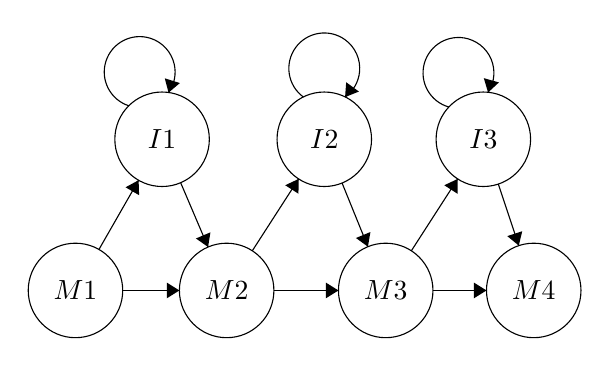
\begin{tikzpicture}[scale=0.2]
\tikzstyle{every node}+=[inner sep=0pt]
\draw [black] (10.7,-27.3) circle (3);
\draw (10.7,-27.3) node {$M1$};
\draw [black] (20.3,-27.3) circle (3);
\draw (20.3,-27.3) node {$M2$};
\draw [black] (30.4,-27.3) circle (3);
\draw (30.4,-27.3) node {$M3$};
\draw [black] (39.8,-27.3) circle (3);
\draw (39.8,-27.3) node {$M4$};
\draw [black] (16.2,-17.7) circle (3);
\draw (16.2,-17.7) node {$I1$};
\draw [black] (26.5,-17.7) circle (3);
\draw (26.5,-17.7) node {$I2$};
\draw [black] (36.6,-17.7) circle (3);
\draw (36.6,-17.7) node {$I3$};
\draw [black] (12.19,-24.7) -- (14.71,-20.3);
\fill [black] (14.71,-20.3) -- (13.88,-20.75) -- (14.74,-21.25);
\draw [black] (14.098,-15.576) arc (252.43495:-35.56505:2.25);
\fill [black] (16.61,-14.74) -- (17.33,-14.13) -- (16.37,-13.83);
\draw [black] (25.177,-15.02) arc (234:-54:2.25);
\fill [black] (27.82,-15.02) -- (28.7,-14.67) -- (27.89,-14.08);
\draw [black] (34.421,-15.655) arc (254.55605:-33.44395:2.25);
\fill [black] (36.9,-14.73) -- (37.59,-14.09) -- (36.63,-13.82);
\draw [black] (13.7,-27.3) -- (17.3,-27.3);
\fill [black] (17.3,-27.3) -- (16.5,-26.8) -- (16.5,-27.8);
\draw [black] (23.3,-27.3) -- (27.4,-27.3);
\fill [black] (27.4,-27.3) -- (26.6,-26.8) -- (26.6,-27.8);
\draw [black] (33.4,-27.3) -- (36.8,-27.3);
\fill [black] (36.8,-27.3) -- (36,-26.8) -- (36,-27.8);
\draw [black] (17.38,-20.46) -- (19.12,-24.54);
\fill [black] (19.12,-24.54) -- (19.27,-23.61) -- (18.35,-24);
\draw [black] (21.93,-24.78) -- (24.87,-20.22);
\fill [black] (24.87,-20.22) -- (24.02,-20.62) -- (24.86,-21.16);
\draw [black] (27.63,-20.48) -- (29.27,-24.52);
\fill [black] (29.27,-24.52) -- (29.43,-23.59) -- (28.51,-23.97);
\draw [black] (32.03,-24.78) -- (34.97,-20.22);
\fill [black] (34.97,-20.22) -- (34.12,-20.62) -- (34.96,-21.16);
\draw [black] (37.55,-20.55) -- (38.85,-24.45);
\fill [black] (38.85,-24.45) -- (39.07,-23.54) -- (38.12,-23.85);
\end{tikzpicture}
\end{center}
	
	Finally, the Viterbi algorithm was run with the query sequence as input, meaning that the most likely sequence of states within the window to have generated the query was calculated.
	
	Then, since gaps were not taken into account in this stage, this positional information was passed on to the next stage, which built a gapped alignment.

	\subsection{\textbf{Simulated Annealing Ungapped Alignment}}
	
	In order to explore the surrounding positions chosen by the HMM's, the HMM's whose found path had the highest likelihood were chosen for further analysis, and the following process was chosen as a way to explore the surrounding space of possible gapped alignments that could be built from the ungapped alignment.
	
	The ungapped alignment produced by the HMM is taken, and is progressively mutated by adding gaps, in order to try and find better alignments. Gaps are inserted as either gaps of three, or gaps of one, and in the testing of this algorithm, the probability of a three gap was set at .99, while a length-one gap was set at .01, in order to represent the relative rarity of frame shift mutations.
	
	At each step, a candidate sequence is produced by adding one of these mutations -- If the resulting sequence is found to be higher scoring than the current best alignment at this position, it is accepted as the new current best, and mutation continued.
	
	If the resulting sequence is not better, it is accepted with a probability according to the following function:
	
	\begin{equation}
		e^{-d/T}
	\label{PAF}
	\end{equation}
	
	Where $d$ is defined as the change in score produced by the move, i.e. the difference between the current stored score and the candidate score.
	
	Additionally, $T$, the temperature, is a set value which is decremented each time a candidate score which is worse than the current score is accepted.
	
	This allows the algorithm to explore suboptimal solutions as it goes on, but it only ever returns the highest scoring alignment it has seen during its exploration of the space, but to a limited extent, as defined by the temperature. Higher values of T will result in a higher likelihood of finding the optimal solution, but at a computational cost.

\section{\textbf{Results: Performance}}

In order to test the algorithm, segments of varying length were randomly sampled from the Boreoeutherian ancestor gene before being mutated through random deletions, insertions, and substitutions, and then used as queries to the algorithm.

\subsection{\textbf{Runtime}}

	In the following tests, the average runtime for a query was measured at approximately five minutes on a machine using two cores of an I5 processor.

\subsection{\textbf{Evaluation}}

	In order to evaluate the performance, we need to define a metric of what a success is for this algorithm. In this context, we are interested in finding the portion of the genome which this sequence came from. Since exactly aligning the sequence is unlikely, we consider the method successful if a candidate solution contains at least 50\% of the original location that generated the query. We also report all candidate solutions which are within a range of 200 positions from the start or stop of the original query, to give an estimate on approximate solutions. A run is successful if the top solution chosen is successful, but we also report a weaker form of success where at least one of the top n candidates is successful.
	
\subsection{\textbf{Accuracy}}

	The following parameter variations are explored:
	\begin{itemize}
	\item Whether or not insertion states are created inside the Hidden Markov Models.
	\item The probability of mutations in the query sequence. Mutation probability of 0, and 0.03.
	\item The word length in the initial ungapped alignment. Word lengths of 6, 8, and 15.
	\end{itemize}
	
	Three query sequences were generated for each of these parameter tests.
	
	Key: A score of \textbf{A} represents the top candidate having at least 50\% of the query within its solution, \textbf{B} represents at least one of the candidates having at least 50\% of the candidate in it, \textbf{C} represents that a candidate solution was within 200 positions from the start or stop of the original query. \textbf{F} represents a complete failure to locate the sequence origin.
	
	\subsection{\textbf{Insertions}}
	
	Three sequences of length 90 were selected with no mutations, and they were given as input to the algorithm with insertions either included or not included. Word size was set to 15, and the HMM window was set to 200.
	
	Overall, no significant difference was found to be caused by the insertion modeling, with most of the top results being almost identical.
	
	
	\begin{table}[htbp]
	\centering
	\caption{Insertion Modeling - No mutations}
	\label{insmod}
	\begin{tabular}{|l|l|l|l|}
	\hline
										 & Q1 & Q2 & Q3 \\ \hline
	Without Insertion: & B  & C  & C  \\ \hline
	With Insertion:    & B  & C  & C  \\ \hline
	\end{tabular}
	\end{table}
	
	\subsection{\textbf{Query Mutations}}
	
	Three sequences of length 90 were selected with mutations, and they were given as input to the algorithm with insertions either included or not included. The other settings were the same as earlier.
	
	\begin{table}[htbp]
	\centering
	\caption{Insertion Modeling - Mutations}
	\label{muts}
	\begin{tabular}{|l|l|l|l|}
	\hline
										 & Q1 & Q2 & Q3 \\ \hline
	Without Insertion: & F  & A  & C  \\ \hline
	With Insertion:    & F  & A  & C  \\ \hline
	\end{tabular}
	\end{table}
	
	\subsection{\textbf{Word Length}}
	
	The word length tests were run with the same default parameters, but with insertions modeled, and mutations at a frequency of 0.05 per position.
	
	As can be seen in the table below, word length had the most significant effect on accuracy for the algorithm.
	
	This is likely due to longer words being more unique, as shorter words were not able to deal with the large number of very similar regions in the genome, meaning that there are many similarly scoring regions for short words, so it does not narrow down the search space accuractely. However, longer words are able to have more unique features, and are thus more discriminative. 
	
		\begin{table}[htbp]
	\centering
	\caption{Word Length}
	\label{wlen}
	\begin{tabular}{|l|l|l|l|}
	\hline
										 & Q1 & Q2 & Q3 \\ \hline
	Word Length 6:     &  F & F  & F \\ \hline
	Word Length 8:     &  F & B  & F  \\ \hline
	Word Length 15:    &  C & A  & C  \\ \hline
	\end{tabular}
	\end{table}

\section{\textbf{Overlap Testing}}
    
    \subsection{\textbf{Experimental Design}}

    In order to further test the algorithm, a larger batch of queries were generated in a similar manner to the earlier queries.
     However, these new queries were generated with an additional layer of complexity in regards to deletions.

     Instead of a deletion occurring on a single character in the query string, deletions of length three were prioritized. 
     This served to more accurately model a system where single nucleotide deletions -- casuing frame shifts -- are much rarer in sequences produced over time.

     If a deletion event triggered on a nucleotide, there was a one percent chance of a single character deletion occurring, and a three nucleotide deletion always occurred otherwise.

    For this experiment, sixty query sequences were generated from random positions within the source genome, and then they were mutated with one percent rates per nucleotide for insertions, deletions, and substitutions. 
    These query sequences were of length 90, and the nucleotides in the sequences were generated according to the probability distributions given in the genome.

    Next, each of these sequences were run through the proposed algorithm, and the results were stored.

    The chosen positions by the algorithm's alignment were compared to the original positions in the generated query, and the percent overlap between the two was calculated.

    Two measures of the overlap were used: 
    First the overlap of all returned alignments for a specific query were averaged and reported, and next, the highest overlap for each query was found and reported for each one. Afterwards, the averages for both of these were calculated.

    The settings used on the algorithm for these experiment were as follows:

    The word size was fifteen, the top six results were returned for the k-length matching and the HMM alignment, and insertions were modelled in the HMM.

    The transition probabilities used for the HMM generation were:
    
    \begin{itemize}
    
        \item Match to Match: .9

        \item Match to Insertion: .1

        \item Insertion to Self: .7

        \item Insertion to Match: .3

    \end{itemize}

    The scores used for alignment evaluation were:
    
    \begin{itemize}
        \item Match: 5

        \item Mismatch: -4

        \item Gap Opening Penalty: -3

        \item Gap General Penalty: -1
    \end{itemize}

    For the simulated annealing step, a starting temperature of twenty was used, and three length gaps were inserted with probability of .99, while one length gaps were inserted with a probability of .01.

    \subsection{\textbf{Data}}

    Presented in the graph below are the results on query sequences labelled 1 through 60, for both the averaged overlap measure, and the maximum overlap measure.

    \includegraphics[width=0.45\textwidth]{overlapchart}

    Additionally, the mean overlap for the averaged overlap measure was 4.9 percent.

    The mean overlap for the maximum overlap measure was 10.4 percent.

    \subsection{\textbf{Discussion}}

    One can quickly see in the above plot that there was a significant portion of queries in which no overlap was found.

    In these cases, it is likely that many of them failed to find any overlap due to the original k-length ungapped alignments failing to identify the correct area in the initial search.

    However, this is not true in all of these cases -- in some of them, the alignment is not correct, but is relatively close (Within 200 nucleotides) of the correct starting position.

    Otherwise, it can be seen that there are a significant number of queries for which overlaps were found. 
    The maximum overlap was generally significantly higher than the overlap of the other alignments produced, which is logical, given that the highest scoring area has many similar sequences which are quite distant from it, meaning that other similar areas could have no overlap at all.

    Additionally, the relatively large number of results with a small proportion of overlap suggests that the alignment step is not accurately aligning the sequence, but is still locating the original location of the query strings in the initial search.

    This means that a portion of the results listed with zero overlap were not in fact totally inaccurate, but certain steps during the pipeline resulted in an inaccurate alignment around the location.

    Even with that issue, a large number of alignments had overlap with the original query.
    
    In fact, $42\%$ of the queries returned a nonzero overlap value, meaning that some portion of the query sequence was within the final alignment, which is a fairly significant result.

    Overall, the algorithm has not returned a reliable result under these settings, but it has certainly performed above chance at identifying these locations, and the techniques used in the algorithm could be adapted in other formats.
	
	
\section{\textbf{Discussion}}

	\subsection{\textbf{Problem Areas}}
	
	When the searches failed completely, it was most likely due to the original k-length ungapped alignments failing to find the correct areas.
	
	Given that there are many locations within the genome that likely look very similar, it is plausible that this could significantly confuse the algorithm, meaning that this makes the algorithm weaker, especially when mutations are involved, as they rule out the ability to make these exact matches, and further obfuscate the location. In BLAST[4], this is addressed by removing low complexity regions, and implementing this could serve as a good extension to test this type of search method.
	
	Additionally, deletions are especially problematic as they are not accounted for in the current HMM structure.

	\subsection{\textbf{Future Improvements}}
	
	One method of improvement which I did not explore is modifying the transition probabilities of the generated HMMs. This could allow a more accurate generation of path likelihood, and help find the exact sequence location. This type of work has been used successfully in work on profile HMMs[1].
	
	It does present other issues though, since directly measuring the transition probabilities as frequencies from something like a probabilistic sequence would require interpreting the probabilities for transitions. 
	
	A similar solution to this as to the original problem could be used, where the frequencies are weighted by the probability of each state involved in the transition.
	
	\subsection{\textbf{Overall Conclusion}}
	
	Though the effect of the Markov Model alignment does not seem promising, the initial evaluation method does accurately locate regions of interest in most cases when used with higher word lengths, and thus the weighting of probability to the scores has a positive effect.

\begin{thebibliography}{00}
\bibitem{b1} Wistrand M, Sonnhammer EL., Improving profile HMM discrimination by adapting transition probabilities, Journal of Molecular Biology, Vol 338(4), pp. 847-54, May 2004.
\bibitem{b2} G. D. Forney, The Viterbi Algorithm, in Proceedings of the IEEE, vol. 61, no. 3, pp. 268-278, March 1973.
\bibitem{b3} Madera M, Gough J., A comparison of profile hidden Markov model procedures for remote homology detection, Nucleic Acids Research, vol. 30, no. 19, pp. 4321-4328, 2002.
\bibitem{b4} Altschul SF, Gish W, Miller W, Myers EW, Lipman DJ, Basic Local Alignment Search Tool, Journey of Molecular Biology, Vol 215, no. 3, pp. 403-410, Oct 1990.
\end{thebibliography}

\end{document}
